%!TEX program = xelatex
\documentclass[xcolor={table}]{beamer}

\usepackage[brazil]{babel}	
\usepackage[utf8]{inputenc}
\usepackage[T1]{fontenc}
\usepackage[scaled]{helvet}
\usepackage{amsthm}
\usepackage{ragged2e}
\usepackage{subfig}
\usepackage[table]{xcolor}
\usepackage{multicol}
\usepackage{multirow}
\usepackage{fancyvrb}
\usepackage{verbatim}
\usepackage{subcaption}

\usetheme{Execushares}

   \begin{subfigure}
           \hspace*{0.1in}

        \vspace*{0.2in}
           
\includegraphics[scale=0.45]{img/URJC_logo.png}
            \label{fig:urjc}
        \end{subfigure}
        \begin{subfigure}
            
\includegraphics[scale=0.36]{img/betsitLogo.png}
            \label{fig:etsit}
        \end{subfigure}

\vspace{0.8cm}
\title{Mejoras en entorno de robótica  educativa para niños}

\subtitle{Trabajo de fin de grado}
\author{Rubén Álvarez Martín}
\date{Noviembre, 2019}

\setcounter{showSlideNumbers}{1}

\begin{document}
	\setcounter{showProgressBar}{0}
	\setcounter{showSlideNumbers}{0}

	\frame{\titlepage}

	\begin{frame}
		\frametitle{Índice}
		\begin{enumerate}
			\item Introducción \\ \textcolor{ExecusharesGrey}{}
		 \textcolor{ExecusharesGrey}{\footnotesize\hspace{1em}}
 		\item Objetivos \\ \textcolor{ExecusharesGrey}{}
		 \textcolor{ExecusharesGrey}{\footnotesize\hspace{1em}}
			\item Herramientas \\ \textcolor{ExecusharesGrey}{\footnotesize\hspace{1em}}
			\item Mejoras a WebSim  \textcolor{ExecusharesGrey}{
			\begin{itemize}
			    \item Soporte a drones en WebSim
			    \item Teleoperadores en WebSim
			    \item Ejercicios individuales
			    \item Ejercicios competitivos  \\
			\end{itemize}} 
			\item Conclusiones  \textcolor{ExecusharesGrey}{\footnotesize\hspace{1em}}
		\end{enumerate}
	\end{frame}

	\setcounter{framenumber}{0}
	\setcounter{showProgressBar}{1}
	\setcounter{showSlideNumbers}{1}
	\section{Introducción}
		\begin{frame}
			\frametitle{Tecnologías web}
			\begin{itemize}
			    \item HTTP
			    \item Tecnologías en cliente
			    \item Tecnologías en servidor
			\end{itemize}
		\end{frame}
			\begin{frame}
			\frametitle{Robótica}

		\end{frame}
		
			\begin{frame}
			\frametitle{Robótica educativa}
			Lenguajes de programación visual:
			\begin{itemize}
				\item \textit{Scratch}
			    \item \textit{LEGO}
			    \item \textit{Kodu}
			    \item \textit{Snap!}
			    \item \textit{Blockly}

			\end{itemize}
		\end{frame}

	\section{Herramientas}
		\begin{frame}
			\frametitle{Herramientas}
\begin{figure}[H]
\centering
\begin{subfigure}{\textwidth}
    
\includegraphics[width=3cm, height=3cm]{img/js.png}
\label{fig:figure2_4}
\end{subfigure}
\begin{subfigure}{\textwidth}
    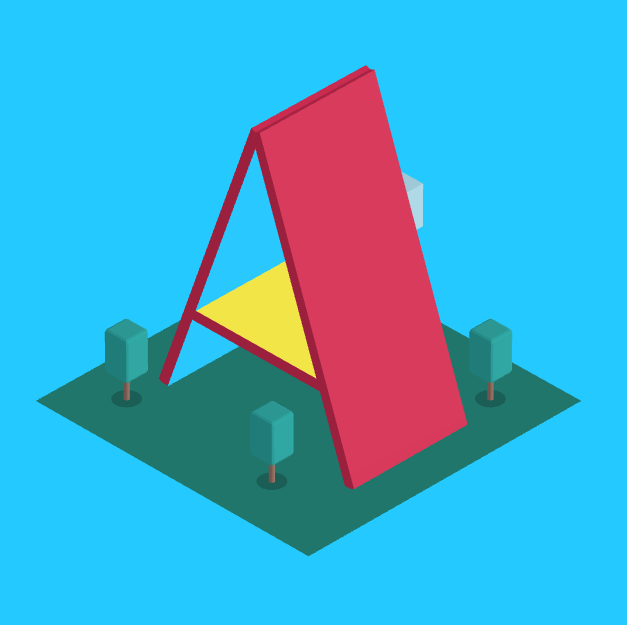
\includegraphics[width=3cm, height=3cm]{img/aframe.png}
\label{fig:figure2_5}
\end{subfigure}\hfill
\begin{subfigure}{\textwidth}
    
\includegraphics[width=3cm, height=3cm]{img/blockly.png}
\label{fig:figure2_6}
\end{subfigure}\hfill
\begin{subfigure}{\textwidth}
    
\includegraphics[width=3cm, height=3cm]{img/blender.png}
\label{fig:figure2_7}
\end{subfigure}\hfill
\begin{subfigure}{\textwidth}
    
\includegraphics[width=3cm, height=3cm]{img/webpack.jpeg}
\label{fig:figure2_9}
\end{subfigure}\hfill
\begin{subfigure}{\textwidth}
    
\includegraphics[width=3cm, height=2cm]{img/npm.png}
\label{fig:figure2_8}
\end{subfigure}\hfill

\label{fig:secuenciaDrone}
\end{figure}
		\end{frame}
			\begin{frame}
			\frametitle{WebSim}
			\begin{itemize}
			    \item \textit{WebSim} es un simulador robótico diseñado para enseñar conceptos básicos de tecnología e iniciar a niños en robótica y programación.
			    
			    \item Permite conectar un editor de texto o bloques a un robot simulado. 
			\end{itemize}
		\end{frame}
		
	\section{Objetivos}
		\begin{frame}
			\frametitle{Objetivos}
			\begin{enumerate}
				\item Ampliar el simulador robótico WebSim para dar soporte a drones
				\item Teleoperadores para poder manejar los robots sin necesidad de programar.
				\item Nuevos ejercicios individuales- Ficheros de configuración y nuevos modelos.
				\item Nuevos ejercicios competitivos y evaluadores automáticos. 
			\end{enumerate}
		\end{frame}

	\section{Mejoras a WebSim}
		\begin{frame}
			\frametitle{Soporte a drones y otros modelos}
				\begin{itemize}
				\item Drivers
				\item Modelo 3D
				\item Bloques 
				\item Otros modelos 
			\end{itemize}
		\end{frame}
			\begin{frame}
			\frametitle{Soporte a drones: Drivers}
				\begin{itemize}
	
			\end{itemize}
		\end{frame}
    	\begin{frame}
			\frametitle{Soporte a drones: Modelo 3D}
				\begin{itemize}
	
			\end{itemize}
		\end{frame}
		   	\begin{frame}
			\frametitle{Soporte a drones: Bloques}
				\begin{itemize}
	
			\end{itemize}
		\end{frame}
		\begin{frame}
			\frametitle{Otros modelos}
				\begin{itemize}
	            \item Fórmula 1
	            
	            \item mBot
			\end{itemize}
		\end{frame}
			\begin{frame}
			\frametitle{Teleoperadores}
	    		\begin{itemize}
				\item Prueba
			
			\end{itemize}
		\end{frame}
		
		
		\begin{frame}
			\frametitle{Teleoperadores: Arquitectura}
			\begin{figure}
			    \centering			    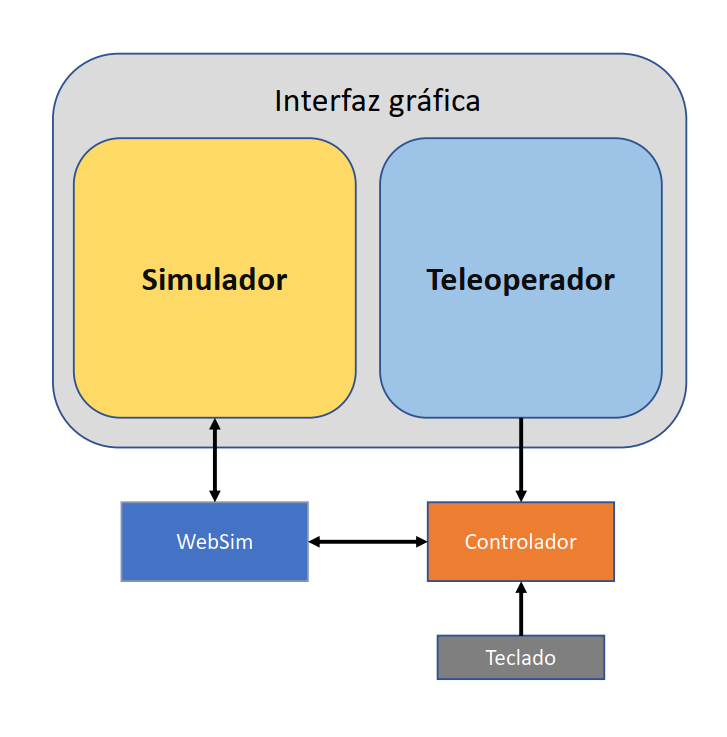
\includegraphics[scale=0.45]{img/arquitecturaTeleoperador.png}
			    \label{fig:teleop}
			\end{figure}
			
		\end{frame}

		\begin{frame}
			\frametitle{Ejercicios individuales}
		\end{frame}
		
		\begin{frame}
			\frametitle{Ejercicios competitivos}
		\end{frame}

	\section{Conclusiones}
		\begin{frame}
			\frametitle{Conclusiones}
			\begin{itemize}
				\item Prueba
			\end{itemize}
		\end{frame}
	
	\appendix

	\backupbegin
	  \begin{frame}
	    \frametitle{Conclusiones}
	  \end{frame}
	\backupend

\end{document}